% fig_fathook.tex -- the fat hook H(a,b) and a dead square (s^s).
% Drawn with a = 2, b = 3, s = 5: the top band is the a unbounded
% rows, the left band the b unbounded columns; the square pokes out
% of both arms.
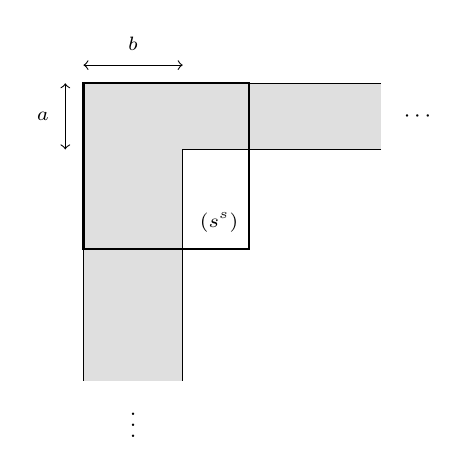
\begin{tikzpicture}[scale=0.42]
  % shaded arms
  \fill[gray!25] (0,0) rectangle (9,-2);
  \fill[gray!25] (0,0) rectangle (3,-9);
  % hook boundary (outer edges and inner staircase)
  \draw (9,0) -- (0,0) -- (0,-9);
  \draw (9,-2) -- (3,-2) -- (3,-9);
  % unboundedness marks
  \node[font=\footnotesize] at (10.1,-1) {$\cdots$};
  \node[font=\footnotesize] at (1.5,-10.1) {$\vdots$};
  % extent markers for a (rows) and b (columns)
  \draw[<->] (-0.55,0) -- (-0.55,-2);
  \node[font=\scriptsize,left] at (-0.75,-1) {$a$};
  \draw[<->] (0,0.55) -- (3,0.55);
  \node[font=\scriptsize,above] at (1.5,0.7) {$b$};
  % the dead square
  \draw[thick] (0,0) rectangle (5,-5);
  \node[font=\scriptsize] at (4.1,-4.2) {$(s^{s})$};
\end{tikzpicture}
